\chapter{Análise e Documentação}
\label{Analise e Documentacao}



\section{Documentação de Requisitos}

A função deste documento é apresentar a descrição de serviços e funcionalidades que o sistema deve possuir, bem como as suas restrições quanto as operações que não é capaz de fazer, servindo como documento base para auxiliar durante as etapas de análise, projeto, testes e homologação do sistema.

    
\subsection{Requisitos Funcionais}
\label{Requisitos Funcionais}
 
 
    \noindent
    \subsubsection{[RF 01] – Realizar login}
    
        O sistema deve permitir que usuários cadastrados com perfil de Administrador realizem \textit{login} com suas credenciais e por meio delas tenha acesso as funcionalidades do sistema.
    
    \noindent
    \textbf{[RF 02] – Redefinir senha}
    
        O sistema deve permitir que o usuário com perfil de Administrador redefina sua senha através do seu e-mail cadastrado. 
    
    \noindent
    \textbf{[RF 03] – Cadastrar usuário}
    
        O sistema permitirá que usuários Administradores cadastrem os usuários que terão acesso ao laboratório. 
    
    \noindent
    \textbf{[RF 04] – Vincular tag a usuário}
    
        O sistema deve permitir no ato do cadastro que o Administrador vincule a tag aproximada no dispositivo embarcado ao usuário cadastrado.
    
    \noindent
    \textbf{[RF 05] – Vincular nova tag a usuário}
    
        O sistema deve permitir que o Administrador vincule uma nova tag a usuários já cadastrados.
        
    \noindent
    \textbf{[RF 06] – Desvincular tag a usuário}
    
        O sistema deve permitir que o Administrador remova a tag vinculadas a um usuário.
    
    \noindent
    \textbf{[RF 07] – Editar usuário}
    
        O sistema deverá permitir que o Administrador edite os dados pessoais do usuário cadastro.
    
    \noindent
    \textbf{[RF 08] – Desativar usuário}
   
        O sistema deverá permitir que o Administrador desative usuários cadastrados no sistema.
        
    \noindent
    \textbf{[RF 09] – Liberar acesso para usuário cadastrado}
    
        A aplicação deve liberar o acesso ao laboratório ao usuário que aproximar a tag do leitor e possuir o cadastro no sistema e a tag vinculada.
    
    \noindent
    \textbf{[RF 10] – Redirecionar usuário não cadastrado para cadastro}
    
        Ao aproximar uma tag do leitor que não possui nenhum vinculo a nenhum usuário o dispositivo embarcado deve exibir no seu LCD uma mensagem redirecionando-o para o Administrador realizar o cadastro do usuário e vinculo a tag.
    
    \noindent
    \textbf{[RF 11] – Visualizar lista de acessos}
    
        Ao Administrador deverá ser permitido a visualização da lista de acessos do laboratório.
    
    \noindent
    \textbf{[RF 12] – Filtrar lista de acessos por período de tempo}
    
        O sistema deverá permitir ao usuário Administrador a busca e visualização da lista de acessos ao usuário por meio da filtragem do período de tempo determinado por ele.
    
    \noindent
    \textbf{[RF 13] – Gerar relatório por período de tempo}
    
        Ao Administrador deverá ser permitido a geração de relatório por meio da busca de acessos pelo período de tempo determinado por ele.


    \subsection{Requisitos Não Funcionais}
    
    \noindent
    \textbf{[NF 01] – Segurança da plataforma}
    
        O sistema deve possuir um sistema de autenticação de modo que apenas usuários com perfil de Administrador tenha acesso ao sistema e suas funcionalidades.
    
    \noindent
    \textbf{[NF 02] – Segurança de acesso}
    
        O sistema deve possuir um sistema de autenticação de modo que apenas tags que possuam vinculo com usuários ativos e validos tenham acesso liberado ao laboratório. 
    
    \noindent
    \textbf{[NF 03] – Sistema Web e linguagem do sistema}
    
        O sistema deve ser desenvolvido em ambiente Web (acesso pelo browser), utilizando linguagem PHP, HTML, CSS e o framework Bootstrap.
    
    \noindent
    \textbf{[NF 04] – Banco de dados}
    
        A cominicação e armazenamento dos dados do sistema deve ser feito por meio do banco de dados MySQL.
        
    

    \subsection{Regras de Negócio}

    \noindent
    \textbf{[RN 01] – Vinculo de tag}
    
        Uma tag deve pertencer apenas a um usuário (usuário pode ter mais de uma tag?).
    
    \noindent  
    \textbf{[RN 02] – Liberar acesso}
    
        O acesso deverá ser liberado apenas para usuários cadastrados que pussuam uma tag vinculada e ativa.
    
    \noindent   
    \textbf{[RN 03] – Visualizar lista de acessos}

        Apenas usuários com perfil de administrador podem ter acesso a lista de acesso e geração de relatório.
    

\section{Artefatos da UML}
    \subsection{Diagrama de Caso de Uso}
    
    \begin{figure}[!hb]
        \centering
        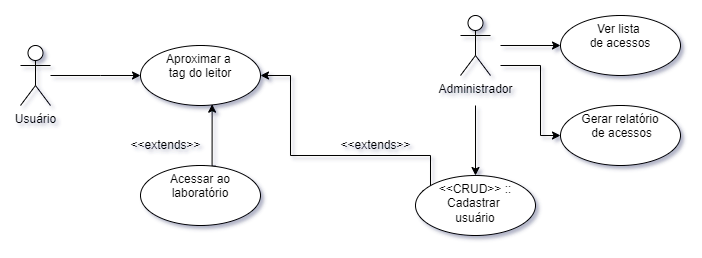
\includegraphics[width=15cm]{images/diagr-caso-de-uso.png}
        \caption{Diagrama de Caso de Uso - IFGAccess}
        \label{fig:diagr-caso-de-uso}
    \end{figure}
    
    \subsection{Descrição dos Casos de Uso}
    
    
\begin{table}[!hb]
\centering
    \begin{tabularx}{0.9\textwidth}{ | >{\raggedright\arraybackslash}X | >{\raggedright\arraybackslash}X | }
        \hline
        \textbf{Nome do caso de uso} & Acessar ao laboratório \\
        \hline 
        \textbf{Atores} &  Usuário \\
        \hline
        \textbf{Requisitos associados} & \\
        \hline
        \textbf{Entradas e pré-condições} & 
        1. O usuário deve estar cadastrado no sistema e a tag deve estar vinculada ao seu perfil \\
        \hline
        \textbf{Saídas e pós-condições} & 
        1. O acesso ao laboratório deve ser liberado
        \newline 2. O sistema grava o horário de acesso do usuário\\ 
        \hline 
        \multicolumn{2}{|l|}{\cellcolor[HTML]{EFEFEF}\textbf{Fluxo de eventos}}  \\
        \hline 
        {\cellcolor[HTML]{EFEFEF}\textbf{Fluxo principal}} & {\cellcolor[HTML]{EFEFEF}}
        1. O usuário aproxima a tag do leitor
        \newline 2. O acesso é liberado
        \newline 3. É registrado o horário de acesso no sistema. \\
        \hline
    \end{tabularx}
    \caption{Descrição de caso de uso 'Acessar ao laboratório'}
    \label{tab:dcu01}
\end{table}

\begin{table}[!hb]
\centering
    \begin{tabularx}{0.9\textwidth}{ | >{\raggedright\arraybackslash}X | >{\raggedright\arraybackslash}X | }
        \hline
        \textbf{Nome do caso de uso} & Cadastrar usuário \\
        \hline 
        \textbf{Atores} &  Usuário e Administrador  \\
        \hline
        \textbf{Requisitos associados} & \\
        \hline
        \textbf{Entradas e pré-condições} & 
        1. O usuário deve aproximar a tag do leitor
        \newline 2. O administrador deve estar logado no sistema web e na tela de cadastro de novo usuário\\
        \hline
        \textbf{Saídas e pós-condições} & 
        1. O cadastro é persistido no banco de dados
        \newline 2. O usuário cadastrado passa a ter acesso ao laboratório\\ 
        \hline 
        \multicolumn{2}{|l|}{\cellcolor[HTML]{EFEFEF}\textbf{Fluxo de eventos}}  \\
        \hline 
        {\cellcolor[HTML]{EFEFEF}\textbf{Fluxo principal}} & {\cellcolor[HTML]{EFEFEF}}
        1. O administrador loga no sistema
        \newline 2. O administrado se direciona a página de cadastro e insere os dados no usuário
        \newline 3. O usuário aproxima a tag do leitor
        \newline 4. A tag reflete na página de cadastro
        \newline 5. O administrador finaliza o cadastro do usuário
        \newline 6. Os dados são persistidos no banco de dados
        \newline 7. É retornando uma mensagem de cadastro efetuado com sucesso no sistema web \\
        \hline
    \end{tabularx}
    \caption{Descrição de caso de uso 'Cadastrar usuário'}
    \label{tab:dcu02}
\end{table}
    
    
    \subsection{Diagrama de Atividade}
    \subsection{Diagrama de Entidade-relacionamento}




\chapter{Resultados}
\label{Resultados}

Este capítulo deve mostrar o que você conseguiu alcançar após aplicar seu método em busca do seu Objetivo.

\section{O que devo escrever aqui?}
Bem, quando você iniciou seu trabalho, você tinha um problema claro a resolver.
Você pesquisou a respeito do seu problema e também a respeito de ferramentas, tecnologias e outros recursos que poderiam ajudá-lo a resolver seu problema. No método você estabelecu os passos usados para resolver o problema. Agora é hora de mostrar em detalhes que você alcançou os objetivos definidos na \nameref{Introducao}.

Oriente-se pelos Objetivos. Descreva em detalhes o seu sucesso!!